% Options for packages loaded elsewhere
\PassOptionsToPackage{unicode}{hyperref}
\PassOptionsToPackage{hyphens}{url}
\PassOptionsToPackage{dvipsnames,svgnames,x11names}{xcolor}
%
\documentclass[
  super,
  preprint,
  3p]{elsarticle}

\usepackage{amsmath,amssymb}
\usepackage{setspace}
\usepackage{iftex}
\ifPDFTeX
  \usepackage[T1]{fontenc}
  \usepackage[utf8]{inputenc}
  \usepackage{textcomp} % provide euro and other symbols
\else % if luatex or xetex
  \usepackage{unicode-math}
  \defaultfontfeatures{Scale=MatchLowercase}
  \defaultfontfeatures[\rmfamily]{Ligatures=TeX,Scale=1}
\fi
\usepackage{lmodern}
\ifPDFTeX\else  
    % xetex/luatex font selection
\fi
% Use upquote if available, for straight quotes in verbatim environments
\IfFileExists{upquote.sty}{\usepackage{upquote}}{}
\IfFileExists{microtype.sty}{% use microtype if available
  \usepackage[]{microtype}
  \UseMicrotypeSet[protrusion]{basicmath} % disable protrusion for tt fonts
}{}
\makeatletter
\@ifundefined{KOMAClassName}{% if non-KOMA class
  \IfFileExists{parskip.sty}{%
    \usepackage{parskip}
  }{% else
    \setlength{\parindent}{0pt}
    \setlength{\parskip}{6pt plus 2pt minus 1pt}}
}{% if KOMA class
  \KOMAoptions{parskip=half}}
\makeatother
\usepackage{xcolor}
\setlength{\emergencystretch}{3em} % prevent overfull lines
\setcounter{secnumdepth}{5}
% Make \paragraph and \subparagraph free-standing
\ifx\paragraph\undefined\else
  \let\oldparagraph\paragraph
  \renewcommand{\paragraph}[1]{\oldparagraph{#1}\mbox{}}
\fi
\ifx\subparagraph\undefined\else
  \let\oldsubparagraph\subparagraph
  \renewcommand{\subparagraph}[1]{\oldsubparagraph{#1}\mbox{}}
\fi


\providecommand{\tightlist}{%
  \setlength{\itemsep}{0pt}\setlength{\parskip}{0pt}}\usepackage{longtable,booktabs,array}
\usepackage{calc} % for calculating minipage widths
% Correct order of tables after \paragraph or \subparagraph
\usepackage{etoolbox}
\makeatletter
\patchcmd\longtable{\par}{\if@noskipsec\mbox{}\fi\par}{}{}
\makeatother
% Allow footnotes in longtable head/foot
\IfFileExists{footnotehyper.sty}{\usepackage{footnotehyper}}{\usepackage{footnote}}
\makesavenoteenv{longtable}
\usepackage{graphicx}
\makeatletter
\def\maxwidth{\ifdim\Gin@nat@width>\linewidth\linewidth\else\Gin@nat@width\fi}
\def\maxheight{\ifdim\Gin@nat@height>\textheight\textheight\else\Gin@nat@height\fi}
\makeatother
% Scale images if necessary, so that they will not overflow the page
% margins by default, and it is still possible to overwrite the defaults
% using explicit options in \includegraphics[width, height, ...]{}
\setkeys{Gin}{width=\maxwidth,height=\maxheight,keepaspectratio}
% Set default figure placement to htbp
\makeatletter
\def\fps@figure{htbp}
\makeatother

\makeatletter
\makeatother
\makeatletter
\makeatother
\makeatletter
\@ifpackageloaded{caption}{}{\usepackage{caption}}
\AtBeginDocument{%
\ifdefined\contentsname
  \renewcommand*\contentsname{Table of contents}
\else
  \newcommand\contentsname{Table of contents}
\fi
\ifdefined\listfigurename
  \renewcommand*\listfigurename{List of Figures}
\else
  \newcommand\listfigurename{List of Figures}
\fi
\ifdefined\listtablename
  \renewcommand*\listtablename{List of Tables}
\else
  \newcommand\listtablename{List of Tables}
\fi
\ifdefined\figurename
  \renewcommand*\figurename{Figure}
\else
  \newcommand\figurename{Figure}
\fi
\ifdefined\tablename
  \renewcommand*\tablename{Table}
\else
  \newcommand\tablename{Table}
\fi
}
\@ifpackageloaded{float}{}{\usepackage{float}}
\floatstyle{ruled}
\@ifundefined{c@chapter}{\newfloat{codelisting}{h}{lop}}{\newfloat{codelisting}{h}{lop}[chapter]}
\floatname{codelisting}{Listing}
\newcommand*\listoflistings{\listof{codelisting}{List of Listings}}
\makeatother
\makeatletter
\@ifpackageloaded{caption}{}{\usepackage{caption}}
\@ifpackageloaded{subcaption}{}{\usepackage{subcaption}}
\makeatother
\makeatletter
\@ifpackageloaded{tcolorbox}{}{\usepackage[skins,breakable]{tcolorbox}}
\makeatother
\makeatletter
\@ifundefined{shadecolor}{\definecolor{shadecolor}{rgb}{.97, .97, .97}}
\makeatother
\makeatletter
\makeatother
\makeatletter
\makeatother
\journal{European Transport Research Review}
\ifLuaTeX
  \usepackage{selnolig}  % disable illegal ligatures
\fi
\usepackage[]{natbib}
\bibliographystyle{elsarticle-num}
\IfFileExists{bookmark.sty}{\usepackage{bookmark}}{\usepackage{hyperref}}
\IfFileExists{xurl.sty}{\usepackage{xurl}}{} % add URL line breaks if available
\urlstyle{same} % disable monospaced font for URLs
\hypersetup{
  pdftitle={CRUSE to Safe Cycling in Ireland},
  pdfauthor={Robin Lovelace; Joey Talbot; Eugeni Vidal-Tortosa; Hussein Mahfouz; Elaine Brick; Peter Wright; Gary O'Tool; Dan Brennan; Suzanne Meade},
  pdfkeywords={Cycling, Open-source, Road Safety, Active Travel},
  colorlinks=true,
  linkcolor={blue},
  filecolor={Maroon},
  citecolor={Blue},
  urlcolor={Blue},
  pdfcreator={LaTeX via pandoc}}

\setlength{\parindent}{6pt}
\begin{document}

\begin{frontmatter}
\title{CRUSE to Safe Cycling in Ireland \\\large{An Open Source Tool to
Support Active Travel} }
\author[1]{Robin Lovelace%
\corref{cor1}%
}
 \ead{r.lovelace@leeds.ac.uk} 
\author[1]{Joey Talbot%
%
}

\author[1]{Eugeni Vidal-Tortosa%
%
}

\author[1]{Hussein Mahfouz%
%
}

\author[2]{Elaine Brick%
%
}

\author[3]{Peter Wright%
%
}

\author[2]{Gary O'Tool%
%
}

\author[4]{Dan Brennan%
%
}

\author[4]{Suzanne Meade%
%
}


\affiliation[1]{organization={University of
Leeds},addressline={Institute for Transport Studies, Leeds, LS2 9JT,
United Kingdom},postcodesep={}}
\affiliation[2]{organization={AECOM},addressline={Unit 6, Galway
Technology Park, Parkmore, Galway, Ireland},postcodesep={}}
\affiliation[3]{organization={AECOM},addressline={Winslade House,
Winslade Park, Manor Drive, Clyst St Mary, Exeter, EX5 1FY,
UK},postcodesep={}}
\affiliation[4]{organization={Transport Infrastructure
Ireland},addressline={Parkgate Business Centre, Parkgate Street, Dublin
8, D08 DK10, Ireland},postcodesep={}}

\cortext[cor1]{Corresponding author}









        
\begin{abstract}
Legislation mandates improved road safety and decarbonisation of
predominantly road-based transport network in Ireland and other
countries. The Cycle Route Uptake and Scenario Estimation (CRUSE) Tool
was commissioned to support cycle network planning, safety
interventions, business case development and project evaluation. Cycling
in Ireland represents only 3\% of total modal share as of the latest
Census (2016), but accounts for 20\% of serious injuries and 7\% of all
fatalities. High resolution datasets on baseline and potential cycling
levels are needed to meet Ireland's climate and safety targets.

The CRUSE Tool is based on open source software and reproducible data
science. The resulting web application is available at
\url{https://cruse.bike/}, enabling planners, engineers, and other
stakeholders to make more evidence-based decisions. CRUSE goes beyond
previous work in several important ways. It models networks at high
levels of geographic resolution, simulates a wide range of trips
including recreational, social, shopping and personal trips, in addition
to trips to work and primary, secondary and tertiary education
locations. The tool provides key `denominator' information to enable
reporting of collision rates per billion km cycled.

Another key feature of CRUSE is its use of frequently-updated
OpenStreetMap data for route calculation and ``cycle friendliness''
estimates of all links on the network. CRUSE provides three network
types: the `Fastest' network highlights routes for directness;
`Quietest' prioritises cycle friendliness, and `Balanced' represents a
balance between speed and comfort. Trips are generated based on origin
and destination data from the 2016 Census in combination with modeled
demand data to estimate current and potential future cycling levels at
area, route, and network levels for each county in Ireland.

For investment in cycling to deliver on the huge potential benefits,
cycling must become safer. With growth in the E-bike market, CRUSE will
help inform inter-urban and rural networks to support the transfer of
trips to sustainable modes for longer journeys. Provision of open access
data in a publicly available web tool will address the challenges faced
by counties across Ireland in meeting their sustainability commitments.
The experience of developing a deploying CRUSE are relevant to countries
with sustainable transport policies worldwide.
\end{abstract}





\begin{keyword}
    Cycling \sep Open-source \sep Road Safety \sep 
    Active Travel
\end{keyword}
\end{frontmatter}
    \ifdefined\Shaded\renewenvironment{Shaded}{\begin{tcolorbox}[sharp corners, boxrule=0pt, borderline west={3pt}{0pt}{shadecolor}, enhanced, interior hidden, breakable, frame hidden]}{\end{tcolorbox}}\fi

\setstretch{2}
\newpage{}

\hypertarget{introduction}{%
\section{Introduction}\label{introduction}}

High energy transport systems are a major contributor to climate change,
a leading cause of premature death and injury due to road traffic
collisions, and a cause of disease due to airborne and noise pollutants.
Conversely, evidence-based and effective transport \emph{policies} have
great potential to decarbonize economies, improve public health, and
save lives.

Transport is responsible for 23\% of global greenhouse gas (GHG)
emissions, 70\% of which are from road transport. Nearly nearly half of
these emissions (around 10\% of global emissions) are from passenger
cars \citep{jaramillo2022}. The transport system encourages, enables and
in some cases enforces unsustainable lifestyles. Services that are only
accessible by car lock-in car dependency
\citep{gray2001, shergold2012, motte-baumvol2010}.

Recognizing the growing evidence of such impacts of poorly designed and
performing transport systems, governments in many countries have set
targets and taken actions. In the context of climate, road safety and
physicial inactivity crises, policies to improve transport systems can
be classified according to the `Avoid-Shift-Improve' (ASI) framework
\citep{jaramillo2022}. The ASI framework highlights the importance of
demand reduction (\emph{avoid}ing unnecessary trips), in addition to
mode \emph{shift} to sustainable modes and \emph{improvement} of
existing energy converters, in that order.

Uptake of cycling should be seen in this broader context of transport
decarbonisation \citep{brand2020} and sustainable mobility
\citep{burns2013}. Although cycling uptake appears on the surface to
only relate to the `shift' part of the ASI framework, closer
consideration of the knock-on impacts of cycling uptake shows that it
can also help avoid unnecessary trips \citep{nello-deakin2020}.
Furthermore, highly efficient e-bikes --- which are seeing rapid uptake
in Ireland and other countries --- outperform electric cars, which are
too heavy and expensive. Over-reliance on electric cars could slow the
transition away from car dependency and inadvertently enable ``high
travel lock-in'' \citep{anable2019}. At the European level, the European
Union has a target of reducing GHG emissions by 55\% by 2030, compared
to 1990 levels, and to achieve `net-zero' by 2050 \citep{rosenow2022}.

Regarding road traffic casualties, another deadly consequence of
inefficient transport systems, the Road Infrastructure Safety Management
(RISM) directive (2008/96/EC) requires member states to implement a road
safety management system (RSMS) for all public roads. Specifically,
``Member States shall ensure that the ranking of high accident
concentration sections and the network safety ranking are carried out''
\citep{directiv2008}. Given that `safety' in this context is usefully
quantified as the number of people killed and seriously injured (KSI)
per distance travelled, the directive requires estimation of distance
travelled by mode, down to the road link level. For active modes, about
which there is a paucity of data compared with motorized modes, this is
a major challenge. Better data to inform road safety policies and
interventions is a motivation for the CRUSE Tool outlined in this paper,
and modeling active travel more broadly.

In Ireland, the Road Safety Authority (RSA) has set the target of
halving the number of road traffic deaths and serious injuries by 2030
\citep{national2021}. Doing so while simultaneously enabling rapid
uptake of active modes will require key active travel routes to be
identified and improved.

A proactive approach to the development of cycling policy and
infrastructure is taking place in Ireland. The main frameworks
underpinning these efforts are the Climate Action Plan
\citep{climate2022a}, the National Development Plan, and the National
Roads 2040 strategy \citep{national2023}. These policy frameworks are
backed-up by public support for active travel interventions: while only
3\% of trips in Ireland are made by cycling according to the latest
Census data from 2016 ``83\% of respondents supported enhanced walking
and cycling facilities'' \citep{sustaina2019}.

At the regional level, the recently published Greater Dublin Area
Transport Strategy \citep{greater} reinforces these findings: ``nearly a
quarter of adults cycle at least once a week in the Dublin Metropolitan
Area'' with cycling in the Dublin area taking up to 60,000 cars off the
road today. Extrapolating this on a per population basis across Ireland,
with around 40\% of the population living in Dublin, this suggests that
around 150,000 cars could be removed nationwide just by achieving Dublin
levels of cycling in all counties (notwithstanding existing cycling
trips and differences in trip distances). 7 in 10 trips in Ireland are
by car \citep{national} . Cycling has the potential to replace a large
proportion of these trips: ``A high priority must also be given to
cyclists, because trips by this mode have the potential to replace trips
by private car, most specifically for short to medium distance trips,
but increasingly for longer trips as e-bikes extend the range of this
mode'' \citep{greater}.

Further evidence of the importance of cycling in Ireland \emph{already}
is provided by the National Strategic Objective (NSO) from the National
Development Plan, with €8.6 billion allocated to sustainable transport
infrastructure including public transport and active travel
interventions. Cycle infrastructure will be developed in synchrony with
the BusConnects project, an entire redesign of the bus network in Dublin
and Cork.

It was in this context that Transport Infrastructure Ireland (TII)
commissioned the Cycle Route Uptake and Scenario Estimation (CRUSE)
project. Based on the Propensity to Cycle Tool (PCT) for England and
Wales, the CRUSE Tool was developed to provide evidence on current
cycling levels and future cycling potential nationwide across Ireland.

A key consideration for TII is to ensure both urban and rural Ireland
were targeted for cycling infrastructure, as shown in
Figure~\ref{fig-dublin}. To this end, TII extensively reviewed activity
on Irish Roads and how the road network was being used by commuters,
cyclists, heavy goods vehicles and other road users across the Irish
transport network. The aim was for the tool to provide strong, national,
systematic but locally-specific evidence to monitor cycling friendliness
and safety in Ireland, to ensure strategic alignment with national,
regional and local policies. The open source and publicly available
nature of the tool ensures more inclusive and evidence-based
conversations around cycle network planning between all stakeholders in
the transport planning process.

TII also requires evidence to support monitoring of growth in cycling,
upgrades of existing cycling infrastructure, business case development
and appraisal, and exposure information to estimate crash rates.
Exposure information is a key part of the the European RISM Directive,
for reporting collision rates of vulnerable road users by 2024. These
factors mean that the tool can be seen as an open access `leverage
point', providing key information for and supporting ambitious plans in
many aspects the planning system, from network design to post-build
monitoring \citep{lovelace2020}.

\begin{figure}

{\centering 

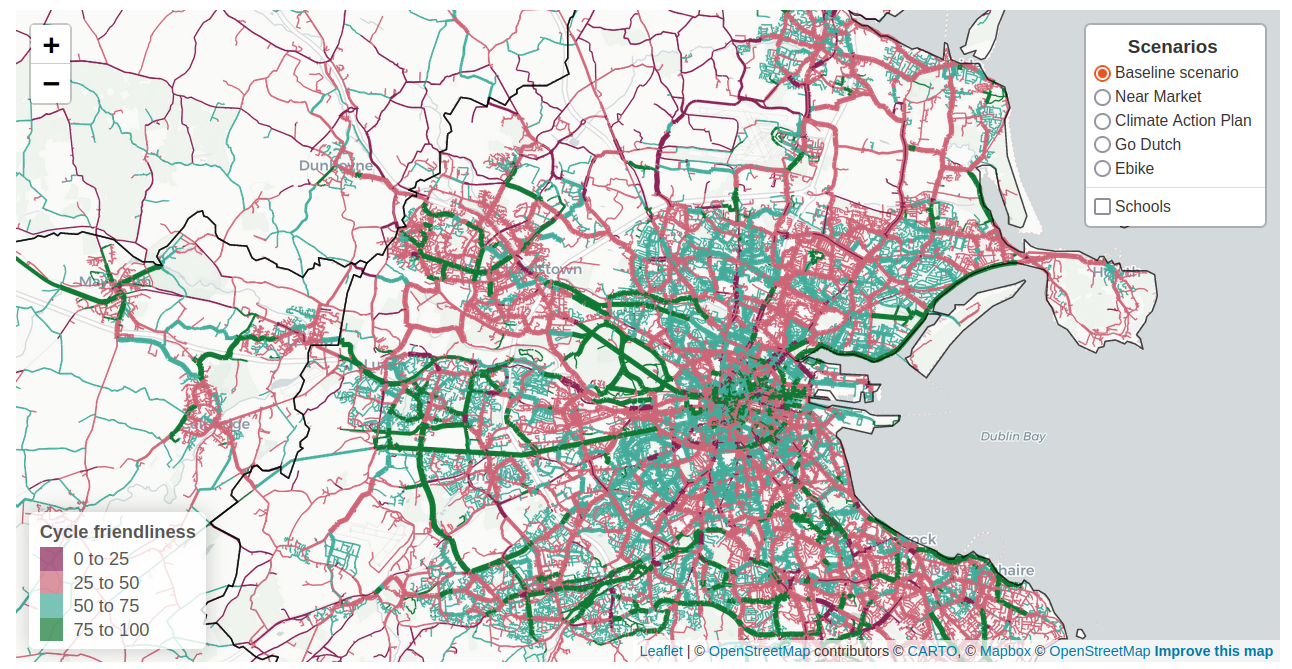
\includegraphics{images/paste-1.png}

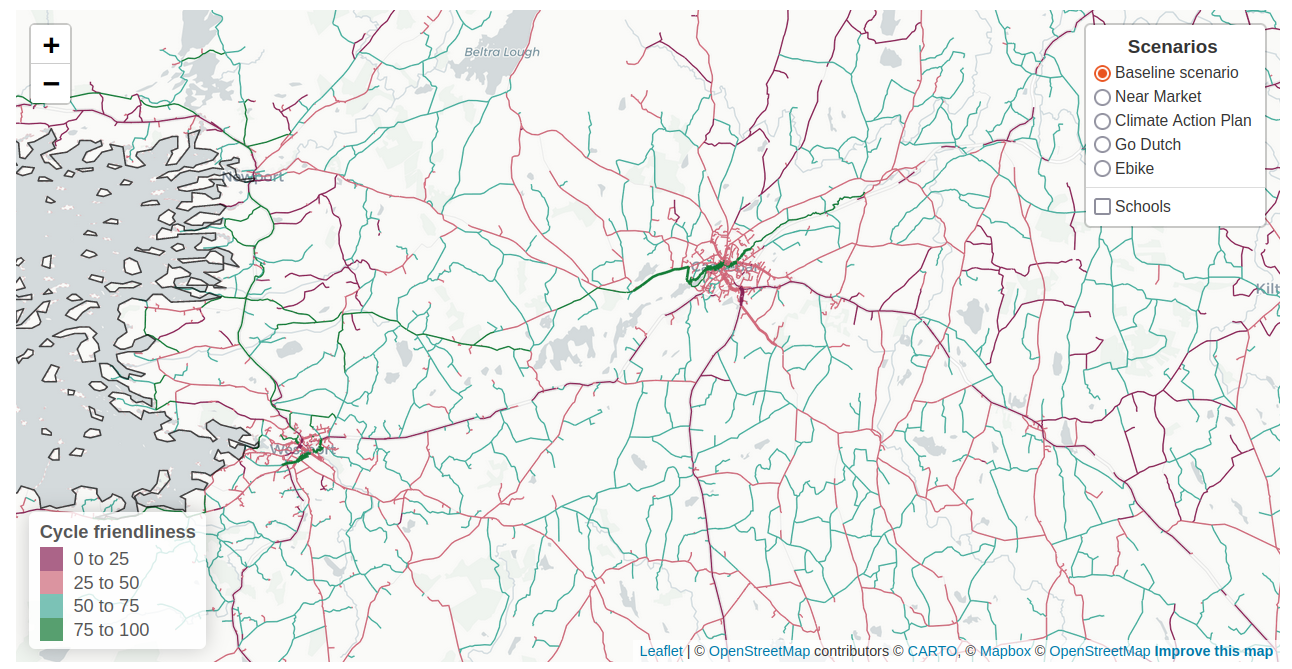
\includegraphics{images/paste-3.png}

}

\caption{\label{fig-dublin}Illustration of the density of route networks
generated by the CRUSE Tool for Dublin City and surroundings (top) and
rural County Mayo on the West coast of Ireland. Source: CRUSE Tool,
available at \url{https://cruse.bike/}.}

\end{figure}

This paper aims to describe the design, features and potential use of
the CRUSE Tool. In Section~\ref{sec-methods}, we outline the methods
used to generate the evidence presented in the CRUSE Tool for Ireland.
In Section~\ref{sec-results}, we present the results of the CRUSE Tool,
including estimates of current cycling levels and future cycling
potential at the national, regional and local levels. In
Section~\ref{sec-discussion}, we discuss the implications of the results
for policy and practice. In Section~\ref{sec-conclusions}, we conclude
the paper.

\hypertarget{sec-methods}{%
\section{Methods and data}\label{sec-methods}}

The methods used to generate the evidence presented in the CRUSE Tool
for Ireland build on the Propensity to Cycle Tool (PCT), which was
originally funded by the UK's Department for Transport and developed by
a multi-university team. An important feature of the PCT is that it is
open source and publicly available (at
\href{https://www.pct.bike/}{www.pct.bike}), allowing its use by all
stakeholders in the transport planning process \citep{lovelace2017}. The
PCT approach has had major policy impacts, as outlined in Research
Excellence Framework (REF) impact case studies, which demonstrate that
the tool ``revolutionised strategic cycle planning in England and
Wales'' by overcoming the barriers to cycling investment imposed by lack
of evidence on cycling potential\citep{lovelace2023}.

The first version of the PCT was based on current and future potential
uptake of cycling for single stage \emph{travel to work} at desire line,
zone, route, and route network levels \citep{lovelace2016}. It was
launched in April 2017 as the government-endorsed tool for strategic
cycle network planning and part of the Cycling and Walking Investment
Strategy \citep{cycling2017}. Extensions of the PCT approach have
included estimation of benefits at the individual level
\citep{woodcock2018}, addition of travel to school network
\citep{goodman2019}, and improved modelling of impacts on health,
environmental and distributional outcomes \citep{woodcock2021}.
Initially developed just for England, the PCT was extended to cover all
of Wales (for commuter data only) in 2018.

The PCT approach has been applied in other countries, including Ireland
(the topic of this paper), Scotland, and Portugal. In Portugal the
`biclaR' project, based on methods underlying the PCT, has been
developed and deployed for the Lisbon metro region. The resulting
evidence is available in an interactive web application hosted at
\href{https://biclar.tmlmobilidade.pt}{biclar.tmlmobilidade.pt}
\citep{felix2023}. biclaR includes estimates of impacts, using the World
Health Organisation (WHO) `HEAT for Cycling' tool and an `intermodality'
scenario that combines cycling with currently available public transit
options based on General Transit Feed Specification (GTFS) data.

The CRUSE Tool seeks to overcome the following methodological
limitations of the original PCT:

\begin{itemize}
\tightlist
\item
  Low resolution of data, with routes starting and ending in
  administrative zone centroids
\item
  Limited coverage of trip purposes beyond travel to work and school
\item
  A web interface that was not user-friendly or intuitive
\end{itemize}

Methods were developed to overcome each of these, as outlined in
Section~\ref{sec-trip-purposes} to Section~\ref{sec-ui}.

\hypertarget{sec-disaggregation}{%
\subsection{Disaggregation of origin-destination
data}\label{sec-disaggregation}}

A feature of active travel interventions is that they require dense
networks of routes to be effective \citep{parkin2018}. This means that
high levels of geographic resolution are needed in the data used to
estimate cycling potential. However, datasets on travel patterns are
often only available at the level of administrative zones. The Central
Statistics Office (CSO) in Ireland provides Place of Work, School or
College Census of Anonymised Records
(\href{https://www.cso.ie/en/census/census2016reports/powscar/}{POWSCAR})
data on the number of people travelling to work and school at the
Electoral Division (ED) level, for example.

The method used to convert OD data to route networks used in the PCT was
to calculate a single route between the population weighted centroids
associated with each OD pair. This method works fine when the OD data
represents movement between small areas, but was not appropriate for
generating route networks from the POWSCAR data because zone centroids
are so far apart that the resulting route networks would be sparse and
unrealistic. To tackle this issue we developed a new method for OD data
disaggregation called `jittering' \citep{lovelace2022}. The method works
by first disaggregating the OD data based on a `disaggregation
threshold' and then assigning each disaggregated `sub-OD' pair to
`subpoints' within each zone. As shown in Figure~\ref{fig-dublin}, the
resulting route networks are dense, even in rural areas.

\hypertarget{sec-trip-purposes}{%
\subsection{Additional trip purposes}\label{sec-trip-purposes}}

A limitation of the original PCT was that it only included travel to
work data. This was partially addressed by the inclusion of travel to
school based on data from the Department for Education in England
\citep{goodman2019}. An advantage of the POWSCAR OD data over OD
datasets derived from census surveys in many countries is that it
includes travel to school data. We commissioned a version of POWSCAR
that included a breakdown of the total flows between OD pairs by purpose
and mode, enabling a more realistic estimation of the `Baseline' cycling
network.

However, travel to school and work only constitute around only 30\% of
all trips in Ireland. To overcome this issue, we developed a spatial
interaction modelling methodology to estimate the number of trips
between each OD pair for additional trip purposes. The classification of
trip purposes used in the CRUSE Tool was guided mainly by the trip
purpose classification found within the National Household Travel Survey
(NHTS), but with the addition of categories based on the comprehensive
POWSCAR data, and the need to include recreational trips and multi-stage
trips (not yet implemented). An overview of the trip purposes used in
CRUSE is presented in Figure~\ref{fig-trip-purposes}.

\begin{figure}

{\centering 

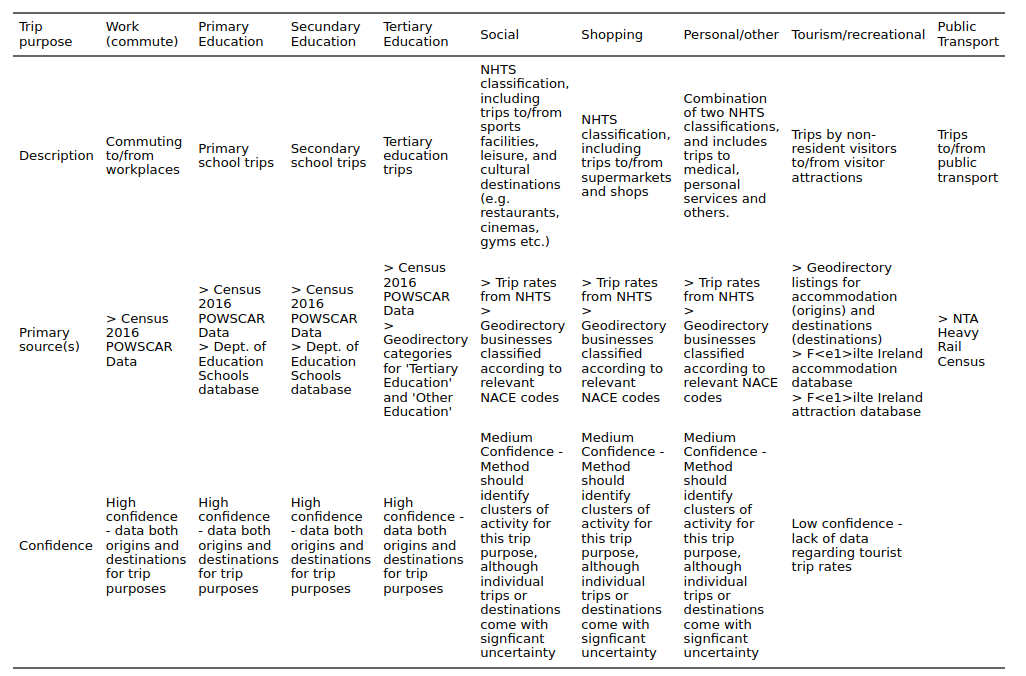
\includegraphics{images/paste-4.png}

}

\caption{\label{fig-trip-purposes}Trip purposes used in the CRUSE Tool.}

\end{figure}

\hypertarget{routing}{%
\subsection{Routing}\label{routing}}

Routes in CRUSE are generated by CycleStreets, a not-for profit
transport consultancy and web development company who provide
application programming interfaces (APIs) supplying a range of datasets
for cycle planning and advocacy. Although based in Cambridge, UK,
CycleStreets provide routing services `by cyclists, for cyclists'
internationally, including in Ireland. The CycleStreets routing engine
is based on OpenStreetMap (OSM) data, which is continuously updated by a
global community of volunteers.

CycleStreets' services can be used by anyone for free, but we
commissioned a bespoke routing service for CRUSE for the following
reasons, to enable:

\begin{itemize}
\tightlist
\item
  Calculation of hundreds-of-thousands of routes, which is beyond the
  terms of service of the free API.
\item
  Making changes to the routing profiles, including allowing routing on
  trunk roads, which are sometimes avoided in the default routing
  profiles.
\item
  Control over the version of OSM data being used for the routing,
  allowing regular updates to the route networks as OSM data is updated.
\end{itemize}

We calculated three network types for each disaggregated (`jittered') OD
pair: `Fastest', `Balanced' and `Quietest'. As outlined on the
CycleStreets'
\href{https://www.cyclestreets.net/help/journey/howitworks/}{website},
the `Fastest' routes minimise journey time, accounting for traffic
lights and surface type. The `Quietest' route type minimises busy
sections of road, allowing high `diversion factors' from the fastest
route on quieter but less direct ways (often avoiding roads and
interactions with motor vehicles altogether where possible). The
`Balanced' route type is a compromise between the two, minimising
journey time while avoiding the busiest roads. Allowing users to switch
between these three route types enables them to consider the trade-offs
between directness and `cycle friendliness' when planning new
infrastructure, as shown in Figure~\ref{fig-route-types}.

These map are available on the `Route types' page for each county (see
\href{https://cruse.bike/kildare/route-types}{cruse.bike/kildare/route-types}).
In addition to showing the estimated routes under each scenario, the
page also presents summary statistics on the network:

\begin{itemize}
\item
  On the fastest network, 25\% of the distance cycled occurs in
  non-hostile segments and 7\% in cycle-friendly segments.
\item
  Under the baseline scenario, 52\% of the distance cycled on the
  quietest network occurs in non-hostile segments and 15\% in
  cycle-friendly segments.
\end{itemize}

These statistics can be revealing: in Kildare it suggests that around
half of all cycling activity occurs on network segments that are hostile
(with a high inferred level of traffic stress), even when efforts are
taken to avoid busy segments. For the Fastest network, which may be more
realistic for utility cycling, the proportion of cycling on hostile
segments is even higher at 75\%.

\begin{figure}

\begin{minipage}[t]{0.50\linewidth}

{\centering 

\raisebox{-\height}{

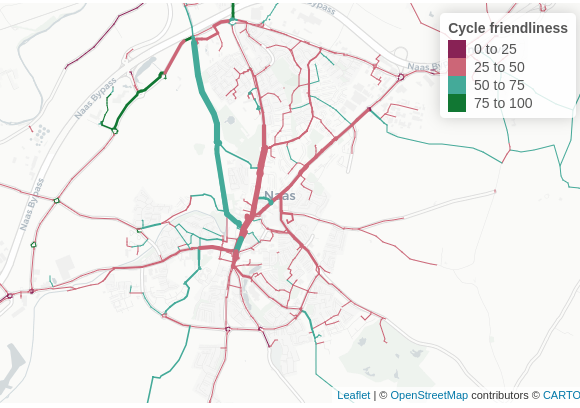
\includegraphics[width=2.60417in,height=\textheight]{images/naas_quietest_godutch.png}

}

}

\end{minipage}%
%
\begin{minipage}[t]{0.50\linewidth}

{\centering 

\raisebox{-\height}{

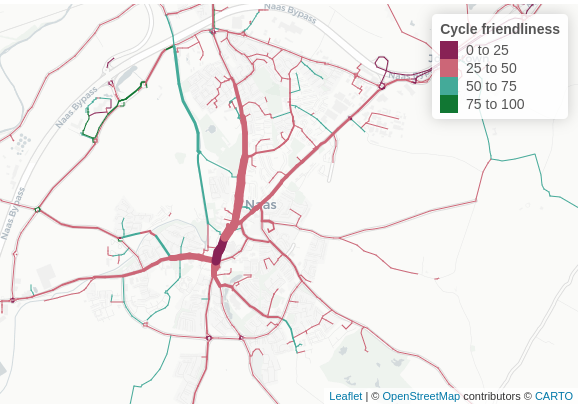
\includegraphics[width=2.60417in,height=\textheight]{images/naas_fastest_godutch.png}

}

}

\end{minipage}%
\newline
\begin{minipage}[t]{0.50\linewidth}

{\centering 

\raisebox{-\height}{

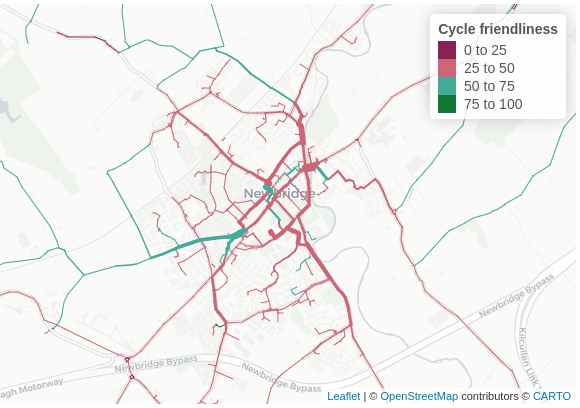
\includegraphics[width=2.60417in,height=\textheight]{images/newbridge_quietest_godutch.png}

}

}

\end{minipage}%
%
\begin{minipage}[t]{0.50\linewidth}

{\centering 

\raisebox{-\height}{

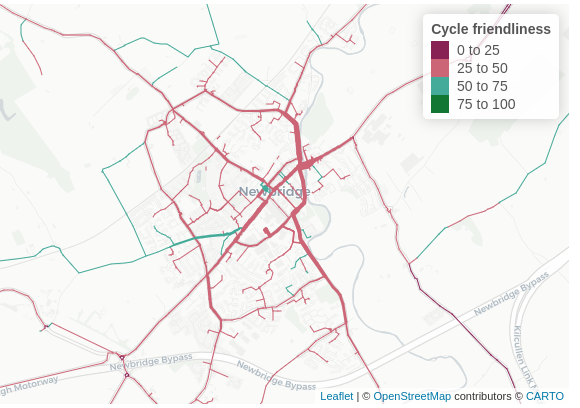
\includegraphics[width=2.60417in,height=\textheight]{images/newbridge_fastest_godutch.png}

}

}

\end{minipage}%

\caption{\label{fig-route-types}Illustration of the Quietest (left) and
Fastest (right) route networks for Naas (top) and Newbridge (bottom).}

\end{figure}

\hypertarget{sec-scenarios}{%
\subsection{Scenarios of cycling potential}\label{sec-scenarios}}

The datasets outlined above were used to generate estimates of cycling
currently (the `Baseline' scenario) and under four scenarios of cycling
potential: Near Market, Climate Action Plan, Go Dutch, and Ebike. Each
of these scenarios is described below, as illustrated in Figure
Figure~\ref{fig-scenarios}.

\begin{figure}

{\centering 

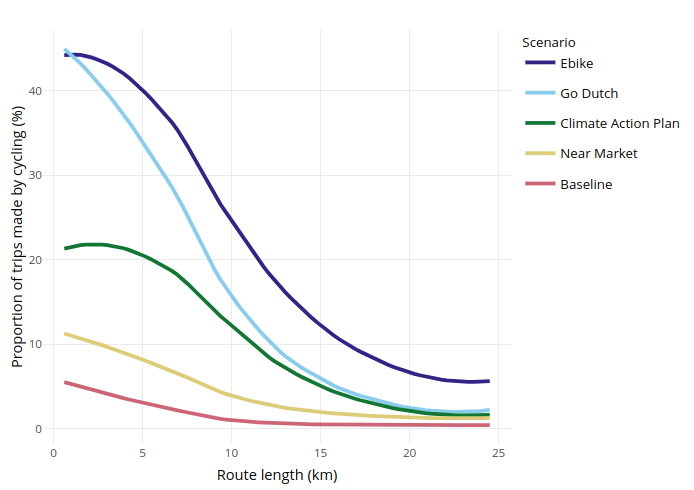
\includegraphics{images/scenarios_kildare.png}

}

\caption{\label{fig-scenarios}Distance-mode share graph for Kildare used
to communicate the different scenarios. Source: county level view for
Kildare in the open access CRUSE Tool at
\url{https://cruse.bike/kildare}.}

\end{figure}

\hypertarget{baseline}{%
\subsubsection{Baseline}\label{baseline}}

The Baseline scenario approximates current cycling levels. As outlined
in Section~\ref{sec-trip-purposes}, the Baseline scenario includes
travel to work and school, and additional trip purposes. Cycling levels
were taken from the POWSCAR data, which includes the number of people
travelling by each mode between each OD pair.

\hypertarget{near-market}{%
\subsubsection{Near Market}\label{near-market}}

The Near Market scenario approximates the level of cycling that would be
achieved if levels of cycling uptake observed in areas of Ireland with
high levels of cycling according to the 2016 Census were achieved
everywhere, accounting for differences in trip distances and hilliness
levels. The scenario is implemented as follows:

\begin{itemize}
\tightlist
\item
  Calculate distance decay curves for Dublin for the base year (2016,
  using POWSCAR data) by fitting a model to the relevant OD data after
  it has been converted to a route network datasest
\item
  Apply the Near Market model to the hilliness and distance values for
  each county during the build process
\item
  Add the current level of cycling to the Near Market model
\end{itemize}

\hypertarget{climate-action-plan}{%
\subsubsection{Climate Action Plan}\label{climate-action-plan}}

The Climate Action Plan scenario is loosely based on the Irish
Government's
\href{https://www.gov.ie/en/publication/6223e-climate-action-plan-2021/}{Climate
Action Plan 2021}, which contains policies for action to achieve a 51\%
reduction in overall GHG emissions by 2030, on a path towards net-zero
by 2050. For transport, this includes 500,000 extra walking, cycling and
public transport trips per day by 2030. In terms of car travel, the
target is to ``Increas{[}e{]} the proportion of kilometres driven by
passenger electric cars to between 40 and 45\% by 2030, in addition to a
reduction of 10\% in kilometres driven by the remaining internal
combustion engine cars.'' This equates to a 5.5 to 6\% reduction in
total car km driven.

To model this decrease in car driver km, cycling uptake increases in
line with the Go Dutch scenario. However, we only model shift from
driving to cycling. There is no shift from other modes of transport to
cycling.

\hypertarget{go-dutch}{%
\subsubsection{Go Dutch}\label{go-dutch}}

Under the Go Dutch scenario cycling reaches levels equivalent to those
found in the Netherlands, taking account of the effects of route
hilliness (measured as mean gradient) and route distance. This scenario
uses the same model that was used PCT, allowing trips to shift from any
other mode to cycling \citep{lovelace2017}.

\hypertarget{ebike}{%
\subsubsection{Ebike}\label{ebike}}

Also based on the PCT scenario with the same name, the Eike scenario in
CRUSE takes Go Dutch cycling uptake, and adds onto this the impact of
increased ebike usage, which allows for longer cycle trips. However,
travel to primary and secondary schools still uses Go Dutch uptake,
since no ebike scenario has been developed for school journeys, and
children may be less likely to own ebikes than adults.

\hypertarget{sec-ui}{%
\subsection{User interface}\label{sec-ui}}

The CRUSE web application is statically hosted, meaning that it can be
accessed without the need for a server running software such as the R
package `shiny' or Python packages such as `streamlit' or `flask' in the
background \citep{wickham2021}. Typical intended user stories are
illustrated in Figure~\ref{fig-user-stories}, which shows that the tool
is designed to be used by both professional and non-professional users.
For the main target audience, professional transport planners working at
the county level, the tool provides a range of outputs, including
estimates of cycling potential at the county and network level. The
provision of balanced (the default), quietest and fastest route networks
enables planners to consider the trade-offs between directness and
`cycle friendliness' when planning new infrastructure. The tool also
provides data downloads, enabling estimates of cycling potential on the
network to be visualised and analysed with other tools such as QGIS,
Python or R.

For non-professional users, the tool provides a simple interface to
explore the cycling potential of the network. By providing a single
landing page that is suitable for both professional and non-professional
users (such as an advocate or parent interested in safe routes to
school), the tool aims to facilitate communication between these groups.

\begin{figure}

{\centering 

\begin{figure}[H]

{\centering 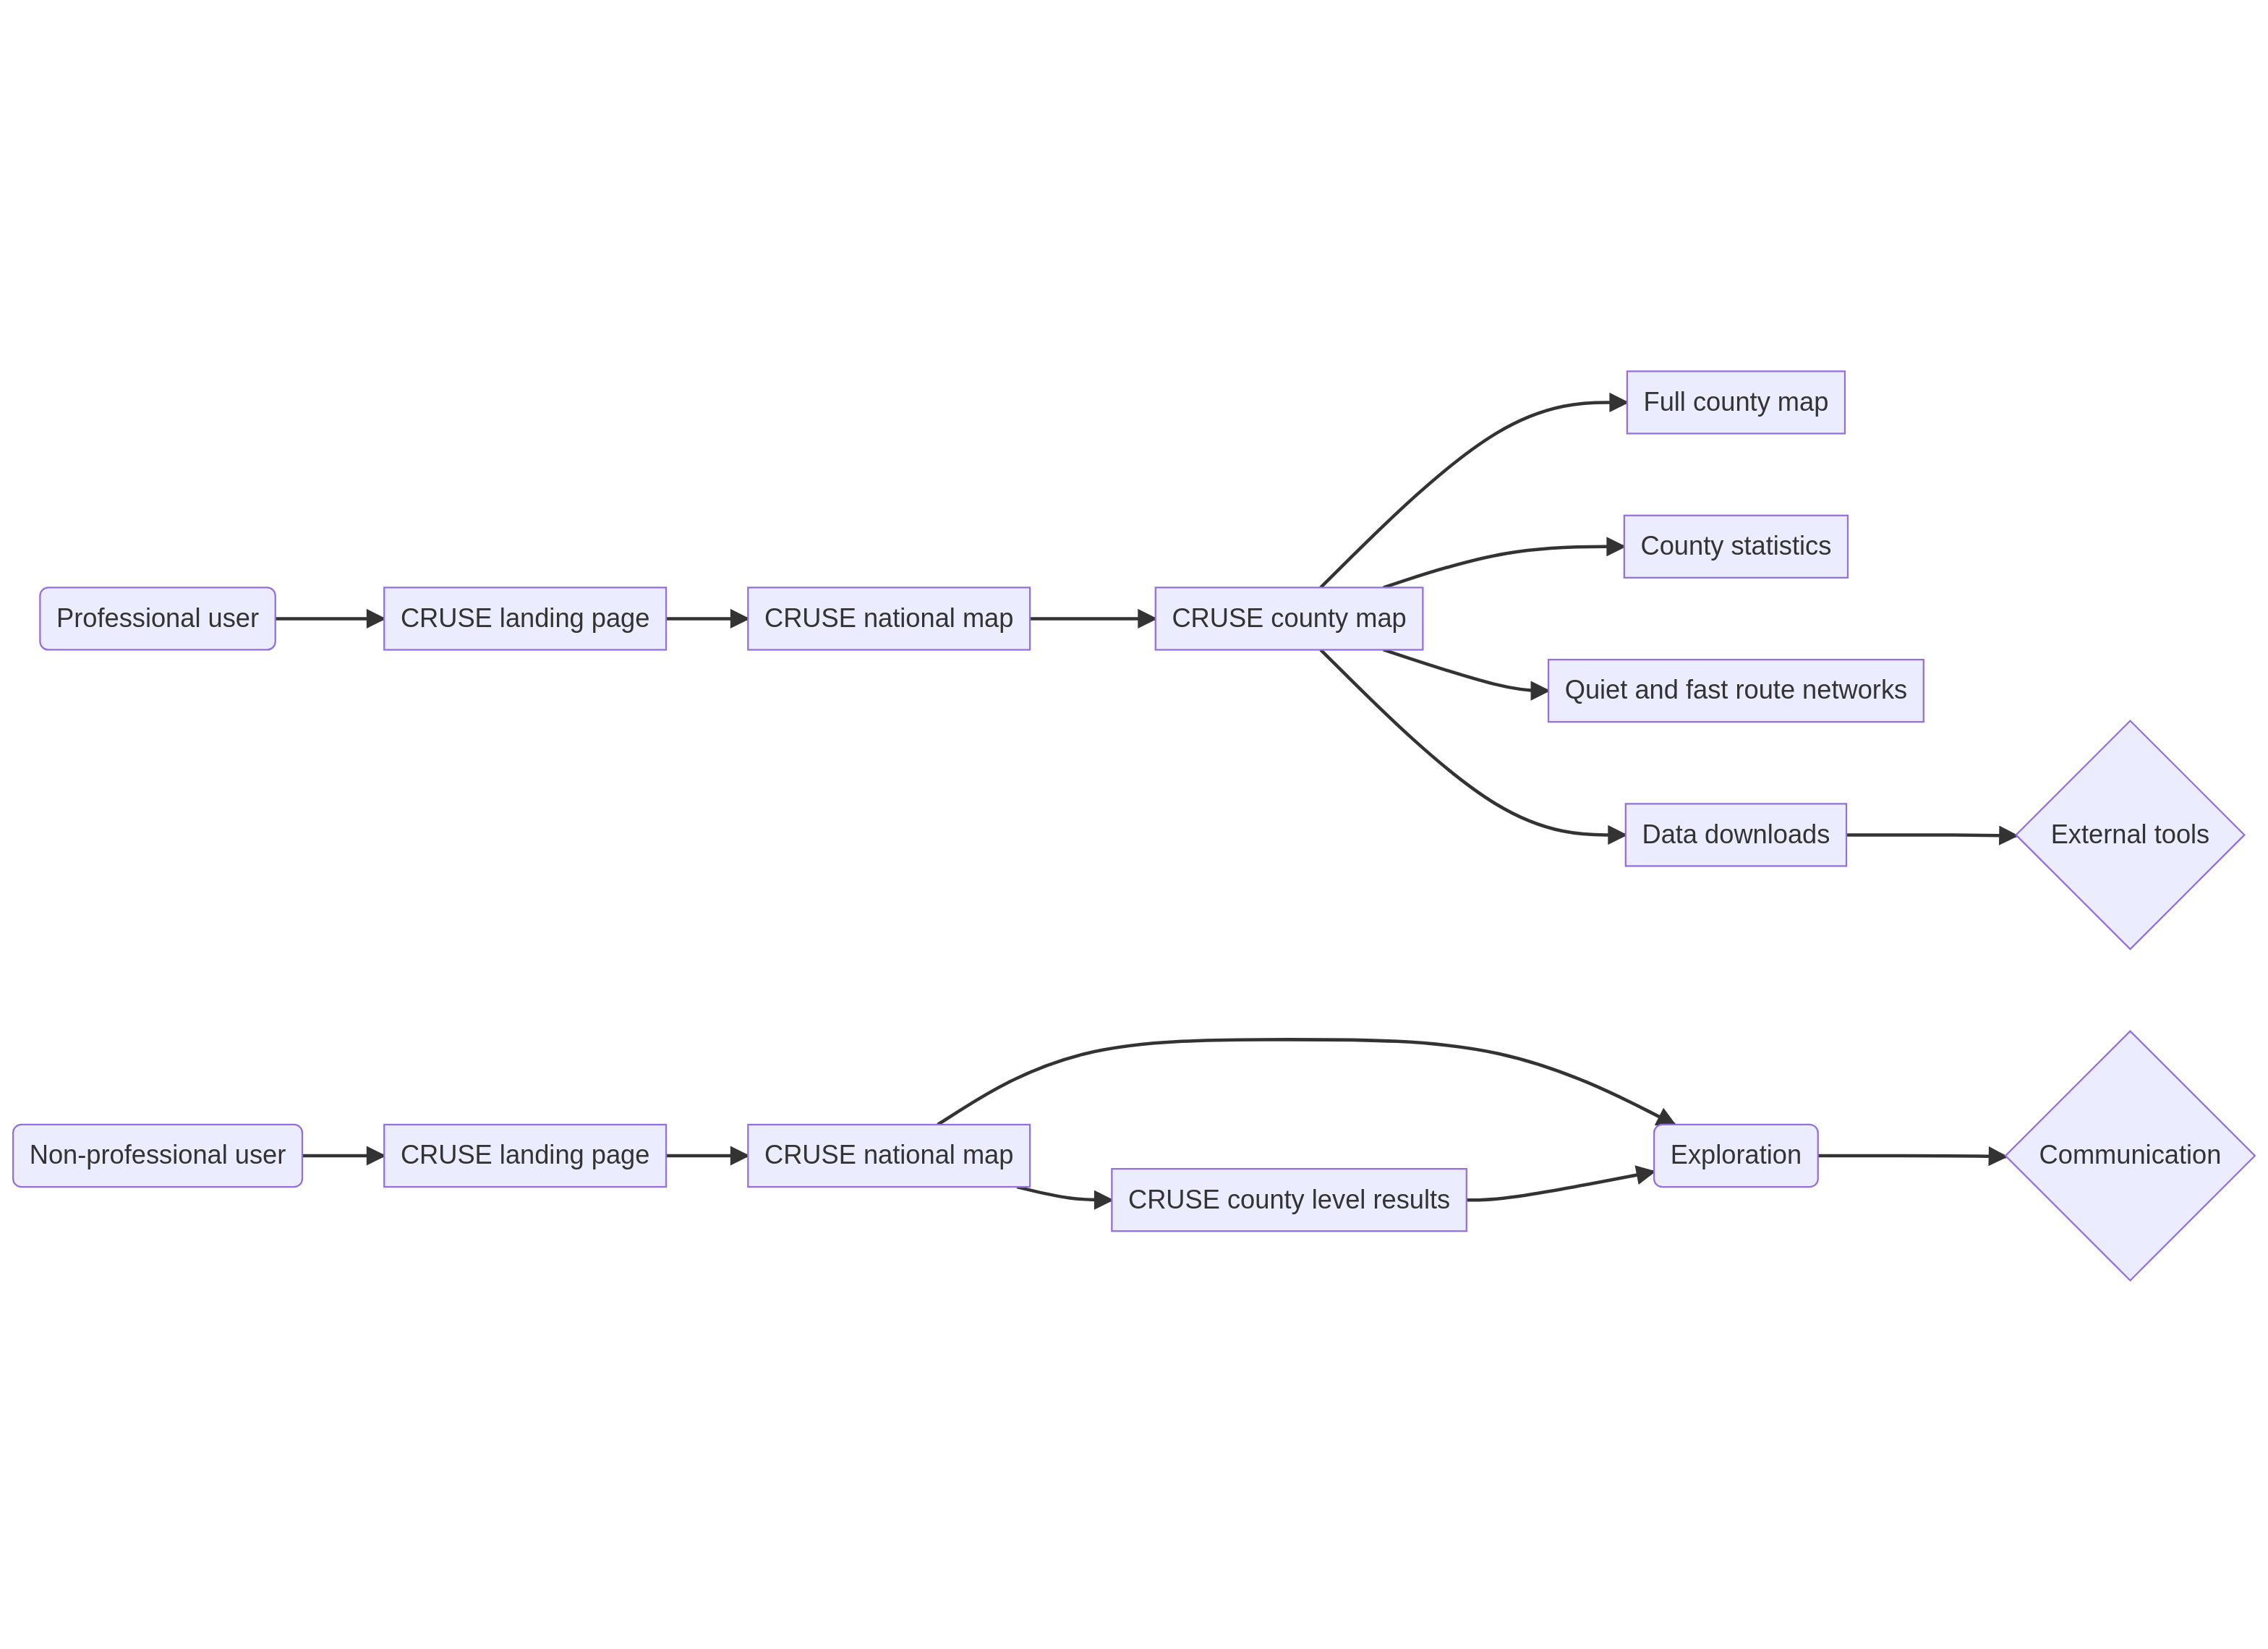
\includegraphics{paper_files/figure-latex/mermaid-figure-1.png}

}

\end{figure}

}

\caption{\label{fig-user-stories}Hypothetical user stories for the CRUSE
Tool illustrating that it can be used in different ways by different
user groups.}

\end{figure}

\hypertarget{sec-results}{%
\section{Results}\label{sec-results}}

The main result of the CRUSE project is an open access web application
and datasets on current and potential future cycling levels in Ireland,
with evidence provided at county and route segment levels. Like the PCT
on which CRUSE builds, a key feature of the results is that they are
systematic and available for all counties, and most routes on which
cycling is permitted, in Ireland. The full set of results are therefore
too extensive to present in their entirety in this paper. Through the
interactive web application, users can explore the data to generate the
results that are most relevant to their needs, whether that is finding
the cycling potential on a particular road or finding `weak links' or
barriers in the cycle network associated with a particular school, work
place or other destination.

Instead of trying to show such use cases, of which there are many
hundreds, we present a selection of results to illustrate the main
features of the CRUSE Tool.

To illustrate the results in urban areas, we took the top 4 cities in
Ireland by population: Dublin City, Cork, Limerick and Galway (with city
populations of 0.6, 0.2, 0.1 and 0.1 million respectively). The results
for central areas demarcated with circular areas with a radius of 3km
for these cities are presented in Figure~\ref{fig-city-results}.

\begin{figure}

{\centering 

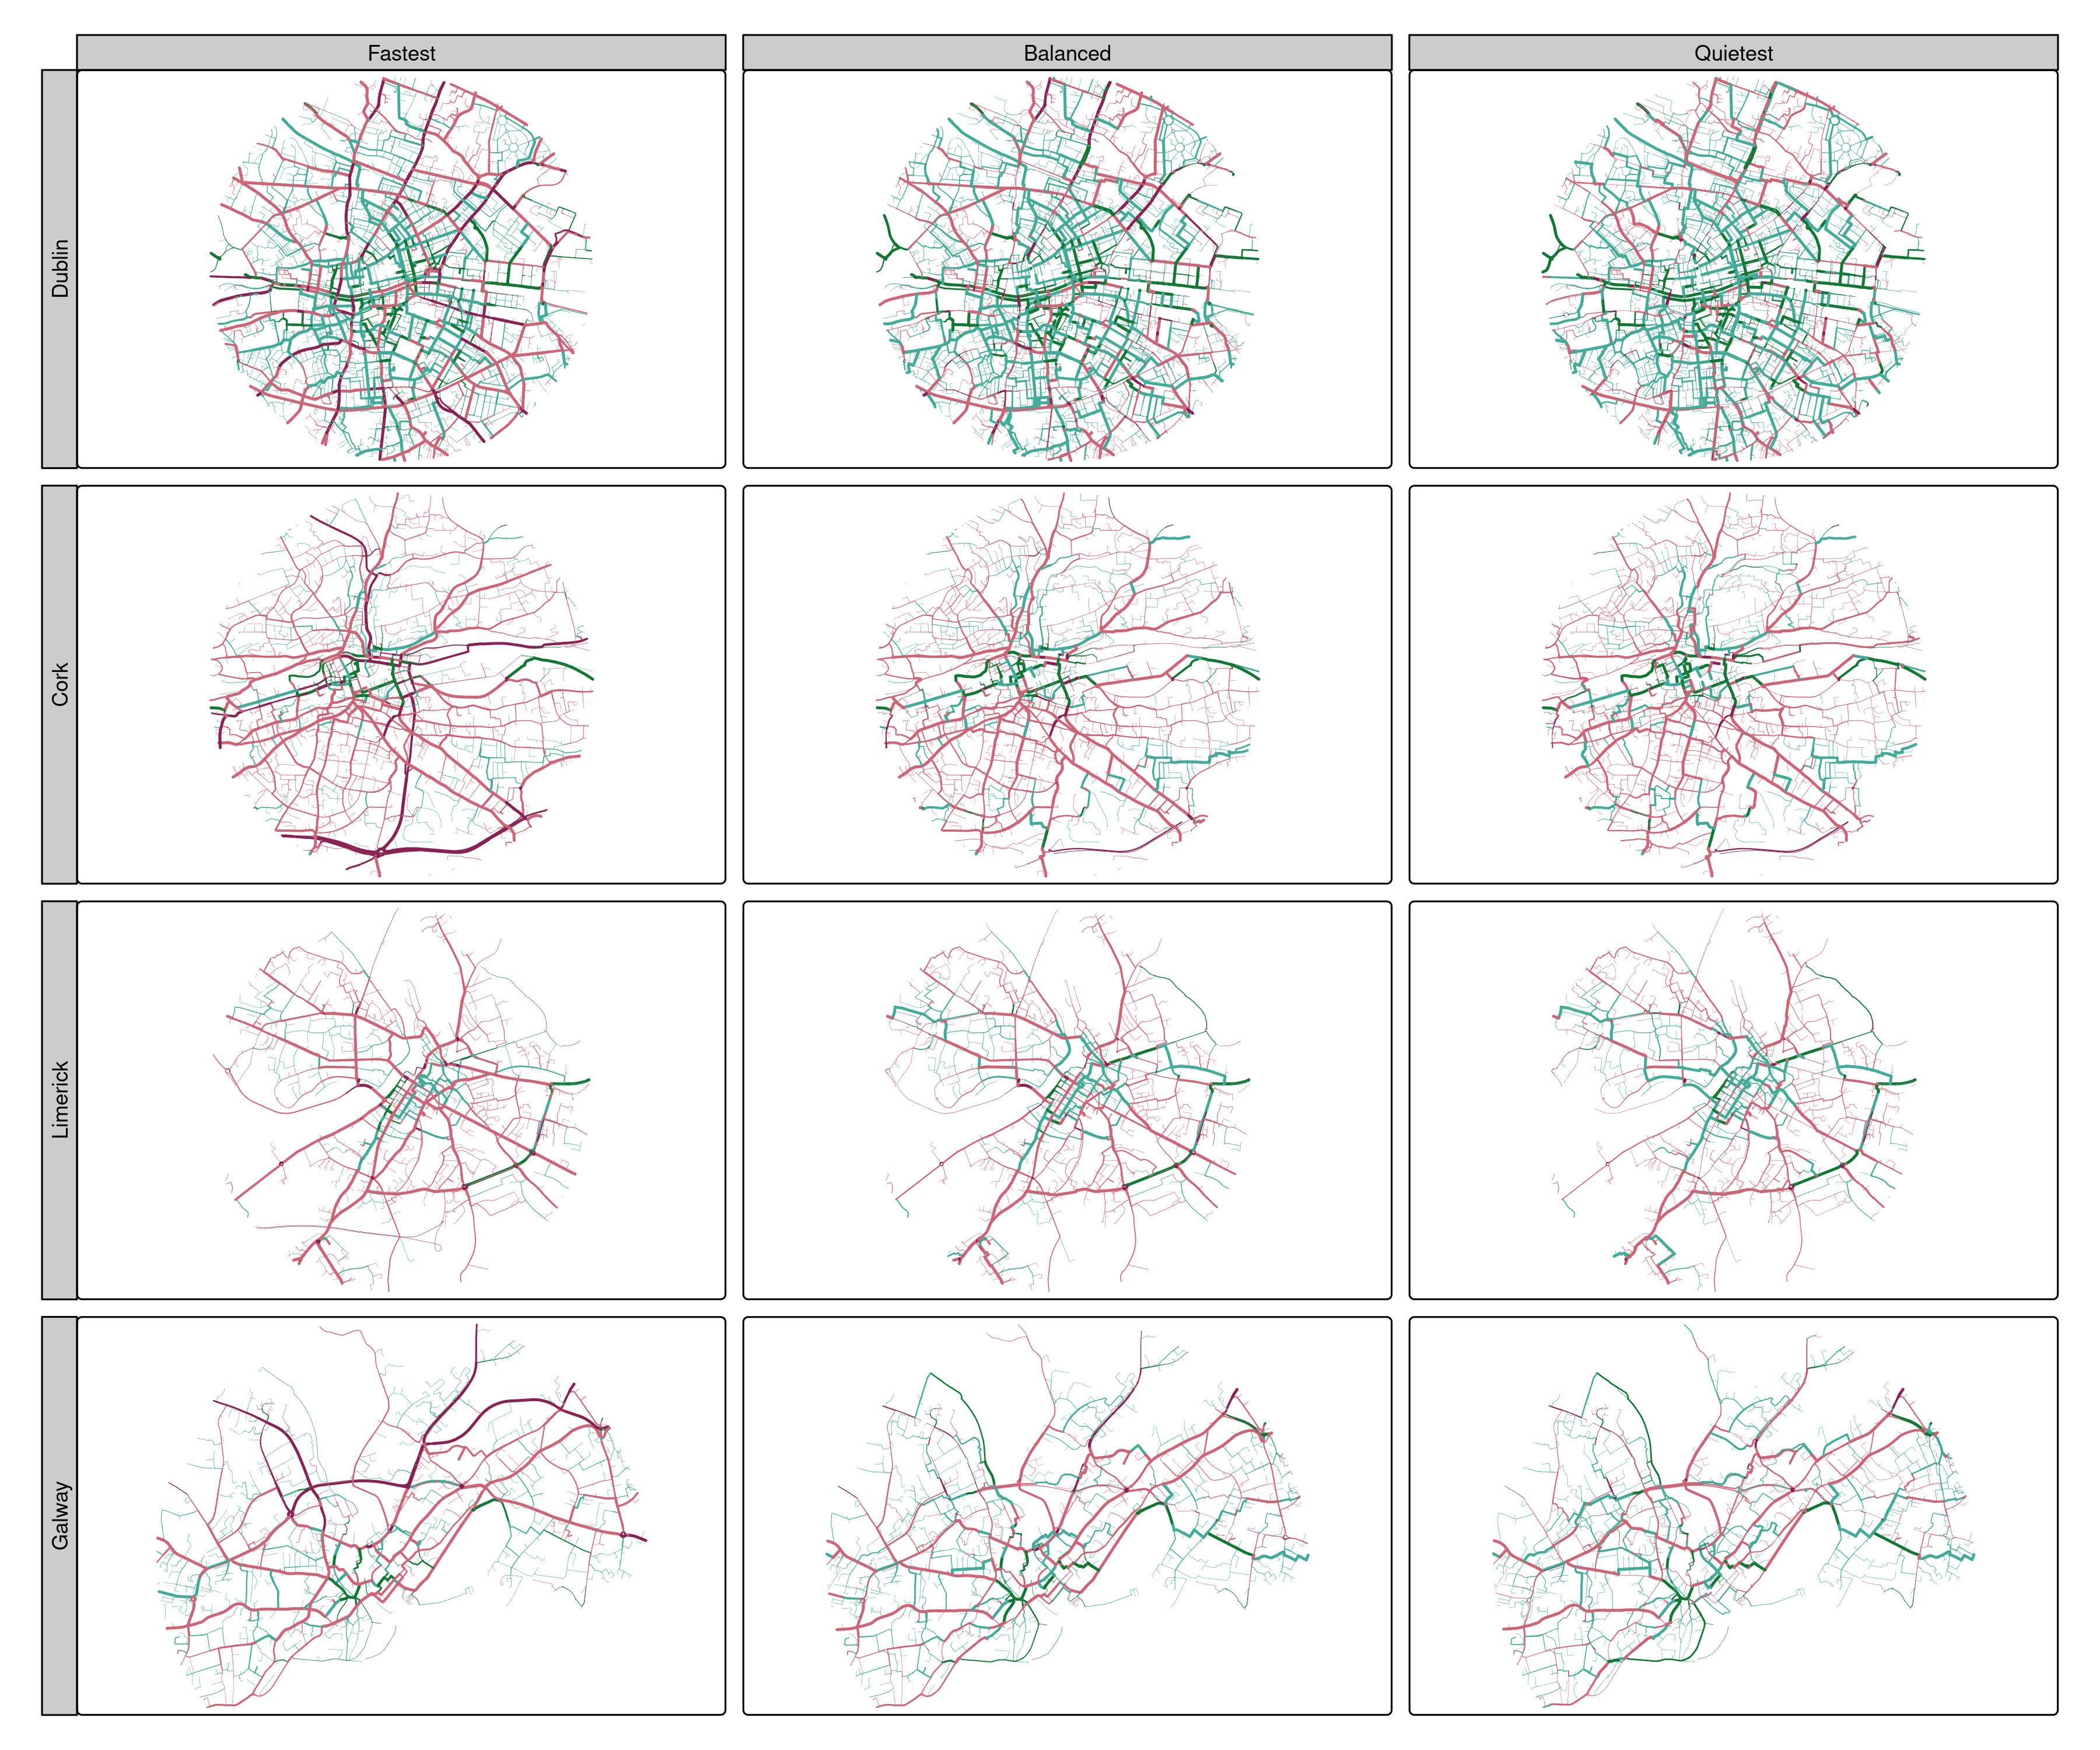
\includegraphics{images/rnet_types.png}

}

\caption{\label{fig-city-results}Fastest, balanced and quietest cycle
networks within 3km circular areas containing the four largest cities in
Ireland. The networks are coloured by cycle friendliness and with widths
varying in proportion to the potential level of cycling under the `Go
Dutch' scenario.}

\end{figure}

Aside from the widely varying sizes and route networks of each city,
with Dublin having by far the densest network, it is clear from the
visualisation of cycling friendliness that there is a lot of room for
improvement in all cities. Dublin has had received most investment in
cycling infrastructure and this is apparent from the high proportion of
the route network that is green, even in the `Fastest' route network
representing routes that prioritise speed and directness over comfort
and safety. Dublin also has the highest mode share of cycling of the
four cities, adding to the evidence base showing that investment in
cycling infrastructure is effective in increasing cycling uptake.

Although Dublin City has made progress, there are still many parts of
the Fastest route network, and even some parts of the Balanced and
Quietest route networks, that are not cycle friendly and which have high
cycling potential. According to a recent report, 71\% of residents in
the Dublin Metropolitan Area support ``more cycle tracks along roads,
physically separated from traffic and pedestrians''.\footnote{https://www.nationaltransport.ie/wp-content/uploads/2022/05/220504-WACI22\_DublinMetropolitanArea\_v35\_DIGITAL\_v2.pdf}
The results for the Dublin area could help prioritise investment in
cycling infrastructure in the city.

\hypertarget{sec-discussion}{%
\section{Discussion}\label{sec-discussion}}

The CRUSE Tool provides evidence on current and potential future cycling
levels across Ireland down to the street level, with potential assigned
to `fastest', `balanced' and `quietest' route networks. This provision
of multiple scenarios of behaviour changes \emph{and} multiple scenarios
of investment, for example in cycling infrastructure next to major roads
vs quiet residential streets, is a key feature of the CRUSE Tool.

As highlighted in a paper on cycling infrastructure preferences based on
a case study of Dublin, both directness and quietness are important
\citep{caulfield2012}:

\begin{quote}
Direct routes with short journey times were found to be the most
important positive variable for existing cyclists and non-cyclists in
determining route choice. This is followed by infrastructure type, the
number of junctions along the route, traffic speed and cyclist volumes.
In terms if infrastructure, regardless of the level of cycling
confidence, routes which have `no facilities' or `bus/cycle lanes' are
the least favoured cycle route types.
\end{quote}

The CRUSE Tool can help both in terms of describing the current
situation, and also prioritise investment in those direct routes with
high cycling potential that lack adequate cycling infrastructure,
highlighted by \citet{caulfield2012}. It will also support reporting for
the RISM Directive on road casualties as part of the road safety
management system.

While the CRUSE Tool is not the first national and publicly available
tool for cycling planning, it has some key features that make it
relevant for other countries, and other national road authorities tasked
with making their transport systems safe:

\begin{itemize}
\tightlist
\item
  The results are \emph{open access} meaning that any stakeholder in the
  planning system can access the evidence. This will help to democratise
  the transport planning process and make wider conversations about
  transport planning more evidence-based and less polarised
  \citep{lovelace2020}, something that is particularly relevant given
  the potentially polarising nature of pro-cycling interventions
  \citep{wild2017}.
\item
  The results are fully reproducible (code to be released pending
  sign-off by TII's IT team), preventing `cloud lock in' to a
  potentially monopolistic consultancy, and encouraging input from the
  wider open source community \citep{lovelace2021, dhir2017}.
\item
  By covering a wide range of trip purposes --- not just travel to work
  \citep{lovelace2017, heinen2010} and travel school \citep{goodman2019}
  as covered in previously published research on open access national
  cycle netework planning tools --- the results capture a higher
  proportion of cycling potential including key rural trips which are
  often under-represented in models of active travel.
\end{itemize}

\hypertarget{sec-conclusions}{%
\section{Conclusions}\label{sec-conclusions}}

The CRUSE Tool is an open access web application for strategic cycle
network planning and prioritisation of road safety interventions across
Ireland. Building on previous work, it provides a nationally consistent
evidence base, providing valuable insights to planners and other
stakeholders in the transport planning process, at national and local
levels. Because the results are available at the route segment level,
the tool can be used to identify `weak links' in the cycle network, and
to prioritise investment in cycling infrastructure. Furthermore, the
provision of the evidence in a free and publicly available website,
hosted at \href{https://cruse.bike}{cruse.bike}, means that it can be
used by anyone, encouraging wider participation and more evidence-based
debate about transport planning.

A key feature of the project methodologically is its calculation of
current and future potential not only for travel to work and travel to
school, but also for other trip purposes, including recreational trips.
This required the development of spatial interaction models and
estimation of the relative attractiveness of different destinations for
different trip purposes, an area of active research where new
developments could be incorporated into the tool in future
\citep{hasova2022}.

The CRUSE Tool and the underlying research and methods are not without
limitations, suggesting future areas of research, data collection needs,
and policy application. The route network level results have not been
validated to the extent we had planned at the outset of the project. We
compared route network level results with `ground truth' data from cycle
counter datasets across Dublin to test different network types and to
ensure that additional trip types added to work and educational trips
increased the quality of fit under the baseline scenario. However, the
size of the counter network was insufficient to provide an opportunity
for robust evaluation of model performance, suggesting a combined
program of new count data collection and analysis should be a priority
for future work, with findings feeding directly into work to improve the
outputs of the the CRUSE Tool.

More broadly, the tool's outputs are limited to just one more of active
travel (cycling), ignoring walking and wheeling, including wheelchair
use and a range of wheeled devices such as scooters, bike trailers and
e-cargo bikes that can be used to escort children to school. Sustainable
transport policies should plan for walking, wheeling and cycling, and
there are many co-benefits of broadly defined active travel
interventions that benefit all active modes, such as measures to reduce
heavy motor traffic speeds and volumes in areas and along corridors with
high active travel potential. This raises the question of whether other
active modes should be incorporated into the results using the OD-based
approach outlined in this paper, or whether different modelling
approaches are needed to properly capture the shorter distance trips
typically made by walking \citep{cooper2018}. Furthermore, the estimates
of cycling presented in the CRUSE Tool omit multi-modal trips including
public transport, and omit trip chaining, due to the need to capture a
large portion of cycling potential within the resource constraints of
the project.

The CRUSE Tool is already used in practice to support more ambitious and
data-driven planning for safe cycling routes in multiple counties across
Ireland. We hope that the underlying approach, and the publicly
available evidence provided in the CRUSE Tool itself, provide a basis
for future reproducible research, open source software development into
strategic cycle network planning tools in Ireland and other countries.
Active travel represents a win-win-win for physical activity,
environment, and local economic opportunities. In combination with
broader sustainable mobility measures and policies to reduce motor
traffic speeds and volumes, tools such as CRUSE can support the fast and
fair decarbonisation of transport systems worldwide.

\hypertarget{list-of-abbreviations}{%
\section{List of abbreviations}\label{list-of-abbreviations}}

CSO: Central Statistics Office

CRUSE: Cycle Route Uptake and Scenario Estimation

ED: Electoral Division

GHG: Greehouse Gas

GTFS: General Transit Feed Specification

KSI: Killed and Seriously Injured

NRA: National Road Authority

NRN: National Road Network

OD: Origin-Destination, typically referring to origin-destination data
which contains information on the number of people travelling between
each pair of zones

OSM: Open Street Map

PCT: Propensity to Cycle Tool

POWSCAR: Place of Work, School or College Census of Anonymised Records

TII: Transport Infrastructure Ireland

\hypertarget{declarations}{%
\section{Declarations}\label{declarations}}

\hypertarget{availability-of-data-and-material}{%
\subsection*{Availability of data and
material}\label{availability-of-data-and-material}}
\addcontentsline{toc}{subsection}{Availability of data and material}

Data was obtained from the Central Statistics Office (CSO) and Transport
Infrastructure Ireland (TII) under license and cannot be shared
publicly. The code used to generate the results presented in this paper
is available at https://github.com/cruse-bike.

\hypertarget{funding}{%
\subsection*{Funding}\label{funding}}
\addcontentsline{toc}{subsection}{Funding}

The work was funded by Transport Infrastructure Ireland (TII).

\hypertarget{acknowledgements}{%
\subsection*{Acknowledgements}\label{acknowledgements}}
\addcontentsline{toc}{subsection}{Acknowledgements}

Thanks to Paul MacDonald and Donal Hodgins (Kildare County Council), for
testing early versions of the tool and for their input into the project.
Thanks to Ciaran Maguire, Catherine Swift, and others at AECOM for their
input into the project. Thanks to Martin Lucas-Smith and Simon Nutall
from CycleStreets for their input into the project.

\hypertarget{competing-interests}{%
\subsection*{Competing interests}\label{competing-interests}}
\addcontentsline{toc}{subsection}{Competing interests}

The authors declare that they have no competing interests.

\hypertarget{authors-contributions}{%
\subsection*{Authors' contributions}\label{authors-contributions}}
\addcontentsline{toc}{subsection}{Authors' contributions}

RL led the development of the CRUSE Tool, with input from JT, EV, HM,
EB, PW, GOT, DB, and SM. SM instigated the project and coordinated its
policy impact. PW, EB and GOT provided project management and transport
engineering expertise.


  \bibliography{bibliography.bib}


\end{document}
